\section[تمرین اول: پیش‌بینی فروش فیلم (\lr{CSM Dataset})]{\faFilm\ \ تمرین اول: پیش‌بینی فروش فیلم (\lr{CSM Dataset}) با رگرسیون خطی}

\begin{stepbox}

\field{هدف و ساختار کلی آزمایش}{
هدف این تمرین، پیش‌بینی میزان فروش ناخالص فیلم‌ها (\lr{Gross}) است. برای درک عمیق‌تر اثر فرآوری داده‌ها، کل فرآیند را به \textbf{دو رویکرد کاملاً متفاوت} تقسیم کرده و نتایج آن‌ها را به چالش کشیده‌ایم:
\begin{enumerate}
    \item \textbf{رویکرد اول:} ساده‌سازی داده‌ها و پیاده‌سازی ریاضی الگوریتم‌ها از پایه.
    \item \textbf{رویکرد دوم:} غنی‌سازی هوشمند داده‌ها (مهندسی ویژگی) و استفاده از پتانسیل کامل ویژگی‌ها.
\end{enumerate}
}

\field{رویکرد اول: تقلیل ابعاد و پیش‌پردازش داده‌ها}{
در این فاز، تمرکز روی پیاده‌سازی دست‌نویس الگوهای ریاضی و کاهش ابعاد داده بود.
\begin{itemize}
    \item \textbf{تحلیل اکتشافی داده‌ها (\lr{EDA}):} با بررسی ماتریس همبستگی، متغیرهای متنی و هم‌خط مثل \lr{Likes, Comments, Views, Dislikes} شناسایی شدند. در مقابل، سه متغیر \lr{Budget}، \lr{Screens} و \lr{Sequel} بیشترین همبستگی را با فروش داشتند.
    \item \textbf{انتخاب ویژگی (\lr{Feature Selection}):} در این گام فقط ۳ متغیر کلیدی فوق حفظ و باقی ستون‌ها حذف شدند.
    \item \textbf{مدیریت داده‌های گمشده:} مقادیر خالی در ستون‌های بودجه و سینماها با الگوریتم \lr{KNNImputer} (با $k=5$) به صورت هوشمند پر شد.
    \item \textbf{تعدیل مقیاس و نرمال‌سازی:} به دلیل نوسان بالا، تبدیل لگاریتمی $\log(1+x)$ روی ویژگی‌های مالی اعمال شد و با روش \lr{Min-Max} به بازه $[0, 1]$ منتقل شدند.
\end{itemize}
}

\field{مدل‌سازی و ساختار ریاضی فرآیند}{
سه مکانیزم برای یافتن بردار وزن بهینه ($\theta$) پیاده‌سازی و مقایسه شد:
\begin{itemize}
    \item \textbf{کاهش گرادیان سنتی (\lr{Gradient Descent}):} با نرخ یادگیری $\alpha = 0.01$ روی تابع هزینه مربعات خطا.
    \item \textbf{بهینه‌سازی با منظم‌سازی \lr{L2} (\lr{Ridge}):} جهت کنترل وزن‌ها با جریمه $\lambda = 1.0$ (بدون اثر روی وزن بایاس):
    \[ J(\theta) = \frac{1}{2m} \left( \sum_{i=1}^{m} (h_\theta(x^{(i)}) - y^{(i)})^2 + \lambda \sum_{j=1}^{n} \theta_j^2 \right) \]
    \item \textbf{معادله نرمال (\lr{Normal Equation}):} محاسبه تحلیلی و دقیق وزن‌ها برای ارزیابی صحت گرادیان کاهشی:
    \[ \theta = (X^T X)^{-1} X^T y \]
\end{itemize}

\vspace{0.4cm}
\begin{center}
    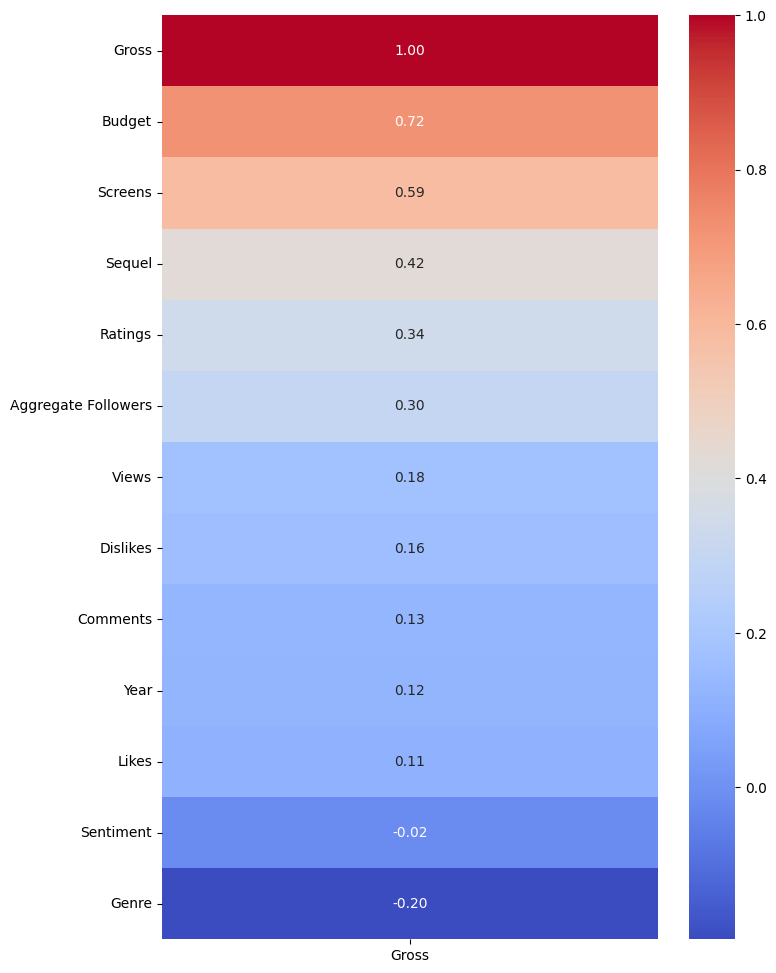
\includegraphics[width=0.5\textwidth]{images/correlation_heatmap.png}
    \captionof{figure}{ماتریس همبستگی متغیرهای منتخب با متغیر هدف (\lr{Gross})}
    \label{fig:correlation_map}
\end{center}
}

\field{نتایج عددی رویکرد اول و چالش بیش‌برازش}{
مقایسه مقدار نهایی تابع هزینه نشان‌دهنده همگرایی دقیق کد دست‌نویس با فرمول تحلیلی است:
\begin{itemize}
    \item هزینه کاهش گرادیان دست‌نویس: $2.179$
    \item هزینه تحلیلی معادله نرمال: $2.080$ (بهینه مطلق)
    \item هزینه رگرسیون ریج (\lr{L2}): $2.803$
\end{itemize}
معیارهای ارزیابی مدل اولیه روی داده‌های تست به شرح زیر است:
\[ \boxed{\text{MSE} = 4.327 \quad | \quad \text{RMSE} = 2.080 \quad | \quad R^2 = 0.427} \]

برای بهبود این رویه، رگرسیون چندجمله‌ای (\lr{Polynomial}) در درجات مختلف ارزیابی شد. همان‌طور که در جدول زیر مشهود است، افزایش درجه مدل به شدت باعث بروز وضعیت \textbf{بیش‌برازش (\lr{Overfitting})} شده است:

\vspace{0.4cm}
\begin{center}
    \captionof{table}{تحلیل خطای رگرسیون چندجمله‌ای به ازای درجات مختلف}
    \label{tab:poly_results}
    \small
    \begin{tabular}{cccc}
    \hline
    \textbf{درجه ($d$)} & \textbf{خطای آموزش (\lr{MSE})} & \textbf{خطای آزمون (\lr{MSE})} & \textbf{وضعیت مدل} \\ \hline
    $\mathbf{d=1}$ & $3.047$ & $4.359$ & پایدار / خطای بالا \\
    $\mathbf{d=2}$ & $3.118$ & $4.355$ & بهینه نسبی \\
    $\mathbf{d=3}$ & $3.309$ & $4.558$ & آغاز بیش‌برازش \\
    $\mathbf{d=4}$ & $3.453$ & $4.732$ & بیش‌برازش شدید \\
    $\mathbf{d=5}$ & $3.520$ & $4.827$ & شکست مدل \\ \hline
    \end{tabular}
\end{center}
}

\field{رویکرد دوم: مهندسی ویژگی پیشرفته}{
در فاز دوم، استراتژی تغییر کرد؛ هیچ داده‌ای دور ریخته نشد و تلاش بر غنی‌سازی متغیرها قرار گرفت.
\begin{itemize}
    \item \textbf{نشانگر باینری برای داده‌های گم‌شده:} به جای پر کردن ساده با میانه، ستون‌های کمکی مثل \lr{\texttt{Budget\_is\_missing}} ساخته شد تا خودِ «فقدان داده» به یک ویژگی یادگرفتنی تبدیل شود و مقادیر اصلی با میانه پر شدند.
    \item \textbf{تحلیل احساسات نام فیلم (\lr{NLP}):} نام متنی فیلم‌ها (\lr{Movie}) با کتابخانه \lr{\texttt{vaderSentiment}} پردازش شد و بار روانی و مثبت/منفی بودن عنوان فیلم به یک معیار عددی پیوسته بین $-1$ تا $+1$ تبدیل و به مدل تزریق گردید.
\end{itemize}
}

\field{نتایج مدل‌های غنی‌شده}{
پس از استانداردسازی داده‌ها با \lr{MinMaxScaler}، نتایج به شکل چشم‌گیری بهبود یافت:
\begin{itemize}
    \item \textbf{مدل \lr{SGDRegressor}:} تنها پس از ۲۳ تکرار با میانگین زیان بسیار پایین $0.012$ همگرا شد و به دقت $R^2 = 0.479$ رسید.
    \item \textbf{مدل رگرسیون خطی استاندارد:} با بهره‌گیری از داده‌های غنی‌شده، جهش بزرگی در عملکرد ثبت کرد و به معیارهای زیر دست یافت:
\end{itemize}
\[ \boxed{\text{MSE} = 2.773 \quad | \quad \text{RMSE} = 1.665 \quad | \quad R^2 = 0.613} \]
}

\field{تحلیل، نتیجه‌گیری و سوال تحلیلی}{
خطای نهایی مدل (\lr{MSE}) از $4.327$ به $2.773$ کاهش یافت و ضریب تعیین ($R^2$) از \%۴۲ به \%۶۱ ارتقا پیدا کرد. این جهش ثابت می‌کند که در مسائل رگرسیون، \textbf{غنی‌سازی داده‌ها (مهندسی ویژگی)} بسیار موثرتر و پایدارتر از پیچیده‌سازی فرمول‌های ریاضی عمل می‌کند.
\vspace{0.4cm}

\textbf{سوال:} آیا می‌توانیم نام فیلم را از مجموعه داده حذف کنیم؟ چرا؟ \\
\textbf{پاسخ:} در رگرسیون خطی سنتی، \textbf{بله}؛ چون مدل‌های رگرسیونی فرمول خطی دارند و رشته‌های متنی خام را نمی‌فهمند. اما از نظر مهندسی ویژگی، \textbf{خیر}؛ دور ریختن کامل نام فیلم اتلاف اطلاعات است. راهکار اصولی این است که مانند رویکرد دوم، ابتدا اطلاعات معنایی یا حسّی آن را استخراج کرده (تبدیل به عدد) و سپس فرمت متنی خام را پاک کنیم.
}

\end{stepbox}